% !TEX encoding = UTF-8 Unicode

%----------------------------------------------------------------------------------------
%	PACKAGES AND OTHER DOCUMENT CONFIGURATIONS
%----------------------------------------------------------------------------------------

\documentclass[twoside]{article}

\usepackage[sc]{mathpazo} % Use the Palatino font
\usepackage[utf8]{inputenc}
\usepackage[english]{babel}
\usepackage[T1]{fontenc} % Use 8-bit encoding that has 256 glyphs
%\linespread{1.05} % Line spacing - Palatino needs more space between lines
\usepackage{microtype} % Slightly tweak font spacing for aesthetics

%\usepackage[hmarginratio=1:1,top=32mm,columnsep=20pt]{geometry} % Document margins
\usepackage[top=20mm,left=8mm,right=8mm,bottom=20mm]{geometry}

\usepackage{multicol} % Used for the two-column layout of the document
\usepackage[hang, small,labelfont=bf,up,textfont=it,up]{caption} % Custom capti
\usepackage{booktabs} % Horizontal rules in tables
\usepackage{float} % Required for tables and figures in the multi-column environment - they need to be placed in specific locations with the [H] (e.g. \begin{table}[H])
\usepackage{hyperref} % For hyperlinks in the PDF

\usepackage{lettrine} % The lettrine is the first enlarged letter at the beginning of the text
\usepackage{paralist} % Used for the compactitem environment which makes bullet points with less space between them

\usepackage{abstract} % Allows abstract customization
\renewcommand{\abstractnamefont}{\normalfont\bfseries} % Set the "Abstract" text to bold
\renewcommand{\abstracttextfont}{\normalfont\small\itshape} % Set the abstract itself to small italic text

%2º espacamento antes da section
\usepackage{titlesec} % Allows customization of titles
%\titlespacing*{\section}{0pt}{0pt}{0pt}
\renewcommand\thesection{\Roman{section}} % Roman numerals for the sections
\renewcommand\thesubsection{\Roman{subsection}} % Roman numerals for subsections
\titleformat{\section}[block]{\large\scshape\centering}{\thesection.}{1em}{} % Change the look of the section titles
\titleformat{\subsection}[block]{\large}{\thesubsection.}{1em}{} % Change the look of the section titles

\usepackage{fancyhdr} % Headers and footers
\pagestyle{fancy} % All pages have headers and footers
\fancyhead{} % Blank out the default header
\fancyfoot{} % Blank out the default footer
\fancyhead[C]{University of Minho $\bullet$ CPD Integrated Project 2015-2016} % Custom header text
\fancyfoot[RO,LE]{\thepage} % Custom footer text

%%% ADDED BY ME %%%%%%
%\floatstyle{boxed} 
\restylefloat{figure}
\usepackage{graphicx}
\usepackage{caption}
\usepackage{subcaption}
\usepackage{amsfonts}
\usepackage{listings,mdframed}
\usepackage{fancyvrb}
\usepackage{cleveref}
\usepackage{mathtools}
\usepackage{amsmath}
\usepackage{color}
\usepackage{relsize}
\usepackage{array}
\newcolumntype{L}[1]{>{\raggedright\let\newline\\\arraybackslash\hspace{0pt}}m{#1}}
\newcolumntype{C}[1]{>{\centering\let\newline\\\arraybackslash\hspace{0pt}}m{#1}}
\newcolumntype{R}[1]{>{\raggedleft\let\newline\\\arraybackslash\hspace{0pt}}m{#1}}
\usepackage{tabularx,caption}
\usepackage{multirow}

%%% For using norm || %%%%%
\newcommand{\norm}[1]{\left\lVert#1\right\rVert}

\newcommand*{\Package}[1]{\texttt{#1}}

\lstset{
    numbers=left,
	language=C,
	keywordstyle=\bfseries\ttfamily\color[rgb]{0,0,1},
	identifierstyle=\ttfamily,
	commentstyle=\color[rgb]{0.133,0.545,0.133},
	stringstyle=\ttfamily\color[rgb]{0.627,0.126,0.941},
	showstringspaces=false,
	basicstyle=\scriptsize,
numberstyle=\tiny,
numbers=right,
	stepnumber=1,
	numbersep=10pt,
	tabsize=1,
	breaklines=true,
	prebreak = \raisebox{0ex}[0ex][0ex]{\ensuremath{\hookleftarrow}},
	breakatwhitespace=false,
	aboveskip={1.5\baselineskip},
  columns=fixed,
  upquote=true,
  extendedchars=true,
 frame=single,
 inputencoding=utf8,
    literate={á}{{\'a}}1 {ã}{{\~a}}1 {â}{{\~a}}1 {é}{{\'e}}1 {ê}{{\'e}}1 {ç}{{\'c}}1 {ú}{{\'u}}1 {ó}{{\'o}}1 {í}{{\'i}}1,
 %backgroundcolor=\color{lbcolor},
}

\usepackage{blkarray}
\usepackage{stmaryrd}

%----------------------------------------------------------------------------------------
%	TITLE SECTION
%----------------------------------------------------------------------------------------

\title{\vspace{-15mm}\fontsize{24pt}{10pt}\selectfont\textbf{Optimisation of a Linear Algebra Approach to OLAP}} % Article title

\author{
\large
\textsc{Filipe Oliveira} - \textsc{A57816}\\
\normalsize \href{mailto:a57816@alunos.uminho.pt}{a57816@alunos.uminho.pt}
\vspace{-5mm}
\and
\textsc{Sérgio Caldas} - \textsc{A57779}\\
\normalsize \href{mailto:a57779@alunos.uminho.pt}{a57779@alunos.uminho.pt}
}



%----------------------------------------------------------------------------------------

\begin{document}

\maketitle % Insert title

\thispagestyle{fancy} % All pages have headers and footers

%----------------------------------------------------------------------------------------
%	ABSTRACT
%----------------------------------------------------------------------------------------

\begin{abstract}
\indent 
\par Online Analytical Processing (OLAP) systems, perform multidimensional analysis of business data and provides the capability for complex calculations, trend analysis, and sophisticated data modelling. 
All the referred analysis depends on Relational Algebra, which lack algebraic properties, and qualitative and quantitative proofs for all the relational operator.
The proposed solution focus on a typed linear algebra approach, encoding OLAP functionality solely in terms of Linear Algebra operations (matrices).
\par It has been argued that linear algebra (LA) is better suited than standard relational algebra for formalising and implementing queries in on-line multidimensional data analysis \cite{macedo2015linear} \cite{da2015benchmarking}. This can be achieved over a small LA sparse matrix kernel which, further to multiplication and transposition, offers the Kronecker, Khatri-Rao and Hadamard products.
We give preliminary experimental results obtained with one cluster of Search6 using queries of the TPC-H Benchmark.
\end{abstract}
\vspace{0.5cm}

%----------------------------------------------------------------------------------------
%	ARTICLE CONTENTS
%----------------------------------------------------------------------------------------
\begin{multicols}{2} % Two-column layout throughout the main article text


% !TEX encoding = UTF-8 Unicode

\section{Introduction}
\indent

The design and development of systems that generate, collect, store, process, analyze, and query large sets of data is filled with significant challenges both hardware and software. Combined, these challenges represent a difficult landscape for software engineers.\par 
The relation database is the current solution 	for big data storage.
Prior efforts have been made \cite{macedo2015linear} \cite{da2015benchmarking} in the research project "Linear Algebra approach to OLAP", in order to fully represent relational algebra in terms of linear algebra operators.
\par Regarding the challenge of High Performance Computing, we implemented from the start a typed linear algebra solution given special importance to the data modelling which, if done poorly, limits the attainable efficiency in data-intesive systems like OLAP.\par 
With respect to performance evaluation and results validation in a real work scenario, the used datasets were produced with TPC-H Benchmark, in which is workload consists of multiple query runs.
In order to obtain realistic and meaningful results large datasets were considered, ranging from 1 to 64GB. 
In order to infer conclusions and compare relational and linear algebra the  object-relational database management system PostgreSQL version 9.6, with roots in open source community, was chosen in order to represent the relational algebra approach. 





\section{Linear Algebra Strategy}
\indent
\subsection{Towards a linear algebra semantics for SQL}

Inspired by point-free relational data processing, an alternative roadmap for parallel online analytical processing (OLAP) can be achieved based on encoding data in matrix format and relying thereupon solely on LA operations\cite{macedo2011middle}. 

\subsubsection{Encoding data in matrix format}

As example of raw data consider the displayed table \ref{table:example_table} where each row records the order key, quantity, return flag, line status and ship date from an given TPC-H benchmark lineitem table. In order to facilitate data association the column number in the corresponding lineitem table was included above each data column.
% !TEX encoding = UTF-8 Unicode

\begin{table}[H]


\caption{ Collection of raw data (adapted from TPC-H benchmark lineitem table). }
\label{table:example_table}
\scriptsize
\centering
\begin{tabular}{ |  L{1.5cm} |  L{1.5cm}  |  L{1.5cm}  |  L{1.5cm}  |  L{1.5cm} |   } 
\hline
\#1	&	\#5	&	\#9	&	\#10	&	\#11	  \\ 
l\_orderkey	&	l\_quantity	&	l\_returnflag	&	l\_linestatus	&	 l\_shipdate 	  \\ \hline
\hline
1	&	17	&	N	&	O	&	1996-03-13	  \\ \hline
1	&	36	&	N	&	O	&	1996-04-12	  \\ \hline
1	&	8	&	N	&	O	&	1996-01-29	  \\ \hline
1	&	28	&	N	&	O	&	1996-04-21	  \\ \hline
1	&	24	&	N	&	O	&	1996-03-30	  \\ \hline
1	&	32	&	N	&	O	&	1996-01-30	  \\ \hline
2	&	38	&	N	&	O	&	1997-01-28	  \\ \hline
3	&	45	&	R	&	F	&	1994-02-02	  \\ \hline
3	&	49	&	R	&	F	&	1993-11-09	  \\ \hline
3	&	27	&	A	&	F	&	1994-01-16	  \\ \hline
\end{tabular}
\end{table}


To obtain useful information from raw data, which in OLAP systems escalated to Terabytes of information, we need to summarise the data by selecting attributes of interest and exhibiting their inter-relationships.\par 
Consider the following simplified TPC-H query 1: "How many items were sold per return flag and line status?". For this particular question, the necessary attributes to answer the query are present on table lineitem, being \textbf{return flag}, \textbf{line status}, and \textbf{quantity}. In relational algebra that question could be easily answered by the following SQL code:

\lstinputlisting[caption=SQL code for the simplified TPC-H query 1, label=simple_query_1]{sql/simple_query_1.sql} %input de um ficheiro


which would produce the result presented on table \ref{table:results_simple_query_1}
% !TEX encoding = UTF-8 Unicode
\begin{table}[H]
\caption{Simplified query-1 result from the collection of raw data (adapted from TPC-H benchmark lineitem table). }
\label{table:results_simple_query_1}
\scriptsize
\centering
\begin{tabular}{ |  L{1.5cm} |  L{1.5cm}  |  L{1.5cm}  |    } 
\hline
\#9	&	\#10		 & \#5	  \\ 
l\_returnflag	&	l\_linestatus	&	 l\_quantity 	  \\ \hline
\hline
N	&	O	&	183	  \\ \hline
R	&	F	&	94	  \\ \hline
A	&	F	&	27	  \\ \hline
\end{tabular}

\end{table}


Aggregations like the presented on the prior simplified query occur in all TPC-H queries, hence performance of group-by and aggregation is quite important. That matter will be addressed in the later sections of the report.\par 
Regarding expressing the OLAP  in therms of LA, the key resides in expressing operations in the form of matrix algebra expressions.  In this particular example, we should be able to build three matrices, one for each attribute, with each matrix being correlated to relational algebra as the row storage of columns \#5, \#9, and \#10. However, in order to do so, we need to find a two-way association between the presented string on the rows \#9 and \#10 and an unique integer identifier. Our proposed solution encodes strings recurring to Gnome \textbf{Gquarks} \cite{gquarks} - a two-way association between a non-zero unsigned int and a char * - based on a thread safe hashtable. \par 
By order of appearance, each unique string will be associated to an unique unsigned integer. Repeated strings will be associated to the prior corresponding unsigned integer. The resulting unsigned integer value range will start in the number 1. The value 0 in GQuarks is associated to NULL. Since in the proposed solution row and column numbers will respect  C-style arrays notation both column and row numbering will start on 0. The GQuark unsigned integer value decremented by 1  will represent the row position on the matrix, and the register number, starting at 0, will represent the column position on the matrix. \par 
We can now verify that at most one non-zero cell can be found in each column the matrix in order to maintain the two-way association between an register and its corresponding string (matrix is "functional"). There is also the possibility of direct associating an register number with a value, wether integer or floating point. The referred matrices will be diagonal matrices, in which the element value is directly associated with the register.\par 
Two types of matrices have now been presented:
\label{definition_matrices}
\begin{enumerate}
\item Projection Matrices - which recur to Gnome Gquarks, in which the Gquark decremented by 1, represents the row position of the matrix, and the register number, starting at 0, will represent the column position on the matrix.
\item Measure Matrices -  direct associating an register number with a value, wether integer or floating point,  which the element value is directly associated with the register number, and consequently the column and row position.
\end{enumerate}
 
We can now build the necessary matrices for the given examples, presented from figure  \ref{fig:example_matrix_5} to \ref{fig:example_matrix_10}. The two-way association between char* and unsigned integer is also presented in table \ref{table:association_quarks_row} in order to aid the example comprehension. 
% !TEX encoding = UTF-8 Unicode
\begin{table}[H]
\caption{Two-Way association between GQuarks and Row Number, for rows \#9 and \#10 presented in the collection of raw data (adapted from TPC-H benchmark lineitem table). }
\label{table:association_quarks_row}
\scriptsize
\centering
\begin{tabular}{ |  L{1.5cm} |  L{1.5cm}  |  L{1.5cm}  |    } 
\hline
String	&	GQuark	&	Row \#	  \\ \hline
\hline
N	&	1	&	0	  \\ \hline
R	&	2	&	1	  \\ \hline
A	&	3	&	2	  \\ \hline
O	&	4	&	3	  \\ \hline
F	&	5	&	4	  \\ \hline
\end{tabular}

\end{table}


  \begin{figure}[H]
    \centering
    \caption{Dense Measure Matrix produced from the collection of raw data (adapted from TPC-H benchmark lineitem table), from column \#5 (quantity column).}
\[
\begin{blockarray}{ccccccccccc}
	&	c0	&	c1	&	c2	&	c3	&	c4	&	c5	&	c6	&	c7	&	c8	&	c9	\\
\begin{block}{c(cccccccccc)}
r0	&	17	&	0	&	0	&	0	&	0	&	0	&	0	&	0	&	0	&	0	\\
r1	&	0	&	36	&	0	&	0	&	0	&	0	&	0	&	0	&	0	&	0	\\
r2	&	0	&	0	&	8	&	0	&	0	&	0	&	0	&	0	&	0	&	0	\\
r3	&	0	&	0	&	0	&	28	&	0	&	0	&	0	&	0	&	0	&	0	\\
r4	&	0	&	0	&	0	&	0	&	24	&	0	&	0	&	0	&	0	&	0	\\
r5	&	0	&	0	&	0	&	0	&	0	&	32	&	0	&	0	&	0	&	0	\\
r6	&	0	&	0	&	0	&	0	&	0	&	0	&	38	&	0	&	0	&	0	\\
r7	&	0	&	0	&	0	&	0	&	0	&	0	&	0	&	45	&	0	&	0	\\
r8	&	0	&	0	&	0	&	0	&	0	&	0	&	0	&	0	&	49	&	0	\\
r9	&	0	&	0	&	0	&	0	&	0	&	0	&	0	&	0	&	0	&	27	\\
\end{block}
\end{blockarray}
 \]
    \label{fig:example_matrix_5}
    \end{figure}
        
\begin{figure}[H]
\centering
\caption{Dense Projection Matrix produced from the collection of raw data (adapted from TPC-H benchmark lineitem table), from column \#9 (return flag column) with 2-way association achieved recurring to GQuarks.}
\[
\begin{blockarray}{ccccccccccc}
	&	c0	&	c1	&	c2	&	c3	&	c4	&	c5	&	c6	&	c7	&	c8	&	c9	\\
\begin{block}{c(cccccccccc)}
r0	&	1	&	1	&	1	&	1	&	1	&	1	&	1	&	0	&	0	&	0	\\
r1	&	0	&	0	&	0	&	0	&	0	&	0	&	0	&	1	&	1	&	0	\\
r2	&	0	&	0	&	0	&	0	&	0	&	0	&	0	&	0	&	0	&	1	\\
\end{block}
\end{blockarray}
\]
    \label{fig:example_matrix_9}
\end{figure}

\begin{figure}[H]
\centering
\caption{Dense Projection Matrix produced from the collection of raw data (adapted from TPC-H benchmark lineitem table), from column \#10 (line status column) with 2-way association achieved recurring to GQuarks.}
\[
\begin{blockarray}{ccccccccccc}
	&	c0	&	c1	&	c2	&	c3	&	c4	&	c5	&	c6	&	c7	&	c8	&	c9	\\
\begin{block}{c(cccccccccc)}
r0	&	0	&	0	&	0	&	0	&	0	&	0	&	0	&	0	&	0	&	0	\\
r1	&	0	&	0	&	0	&	0	&	0	&	0	&	0	&	0	&	0	&	0	\\
r2	&	0	&	0	&	0	&	0	&	0	&	0	&	0	&	0	&	0	&	0	\\
r3	&	1	&	1	&	1	&	1	&	1	&	1	&	1	&	0	&	0	&	0	\\
r4	&	0	&	0	&	0	&	0	&	0	&	0	&	0	&	1	&	1	&	1	\\
\end{block}
\end{blockarray}
\]
\label{fig:example_matrix_10}
\end{figure}
    
    \subsection{Projection Operation}

Regarding the projection statement of the example query:

\lstinputlisting[caption=SQL code for the simplified TPC-H query 1 only for the SELECT and GROUP BY statements, label=simple_query_1_only_select]{sql/simple_query_1_only_select.sql} %input de um ficheiro
 the typical case to reproduce a SELECT and GROUP BY statement on a relational algebra approach would be to remove certain columns of the lineitem table. 
 In the LA approach the process consists of joining the projection matrices of the selected attributes. 
 The final LA result should hold all possible combinations
of the projected attributes and no duplicated tuples. That can be achieved by doing several Khatri-Rao products, one for each tuple of attributes present in the statement.\par 
The corresponding LA encoding of the SQL statement from listing \ref{simple_query_1_only_select} is given by the equation presented in equation \ref{eq:khatri_1}.
 
\begin{equation}
\centering
Projection\ Matrix\ =\ ReturnFlag\ \otimes LineStatus
\label{eq:khatri_1}
\end{equation}

which would produce the matrix presented in figure \ref{fig:example_matrix_krao}.
  
\begin{figure}[H]
\centering
\caption{Projection Matrix produced from the Khatri-Rao product between return flag and line status columns from lineitem table, from columns \#9 and \#10.}
\[
\begin{blockarray}{ccccccccccc}
		& c	0	& c	1	& c	2	& c	3	& c	4	& c	5	& c	6	& c	7	& c	8	& c	9	\\
\begin{block}{c(cccccccccc)}
r	0	&	0	&	0	&	0	&	0	&	0	&	0	&	0	&	0	&	0	&	0	\\
r	1	&	0	&	0	&	0	&	0	&	0	&	0	&	0	&	0	&	0	&	0	\\
r	2	&	0	&	0	&	0	&	0	&	0	&	0	&	0	&	0	&	0	&	0	\\
r	3	&	1	&	1	&	1	&	1	&	1	&	1	&	1	&	0	&	0	&	0	\\
r	4	&	0	&	0	&	0	&	0	&	0	&	0	&	0	&	0	&	0	&	0	\\
r	5	&	0	&	0	&	0	&	0	&	0	&	0	&	0	&	0	&	0	&	0	\\
r	6	&	0	&	0	&	0	&	0	&	0	&	0	&	0	&	0	&	0	&	0	\\
r	7	&	0	&	0	&	0	&	0	&	0	&	0	&	0	&	0	&	0	&	0	\\
r	8	&	0	&	0	&	0	&	0	&	0	&	0	&	0	&	0	&	0	&	0	\\
r	9	&	0	&	0	&	0	&	0	&	0	&	0	&	0	&	1	&	1	&	0	\\
r	10	&	0	&	0	&	0	&	0	&	0	&	0	&	0	&	0	&	0	&	0	\\
r	11	&	0	&	0	&	0	&	0	&	0	&	0	&	0	&	0	&	0	&	0	\\
r	12	&	0	&	0	&	0	&	0	&	0	&	0	&	0	&	0	&	0	&	0	\\
r	13	&	0	&	0	&	0	&	0	&	0	&	0	&	0	&	0	&	0	&	0	\\
r	14	&	0	&	0	&	0	&	0	&	0	&	0	&	0	&	0	&	0	&	1	\\
\end{block}
\end{blockarray}
\]
\label{fig:example_matrix_krao}
\end{figure}

Given the matrices A with dimensions $(m\ \times\ n)$ and B with dimensions $(o\ \times\ p)$, the produced projection matrix has dimensions $(q\ \times\ r)$, being $q\ =\ m =\ o$ and $r = m \times o$. The produced matrix dimensions can also be expressed as $(\ (\ m\ \times\ o\ )\ \times\ n)$ as visible on figure \ref{fig:example_matrix_krao}.\par
In order to produce the desired tuples  holding all possible combinations, the association between row number and tuple has to be created. Given two original matrices A with dimensions $(m\ \times\ n)$ and B with dimensions $(o\ \times\ p)$, and one produced projection matrix C via the Khatri-rao product, in order re-obtain both strings that produce each tuple, for every row R$_{C}$ from the C matrix, the corresponding R$_{A}$ from matrix A, and R$_{B}$ from matrix B, are given by the expression: 


\begin{equation} \label{eq:eq1}
\begin{split}
R_A = R_C / o \\
 R_B\ =\  R_C  \mathbin{\%}  o
\end{split}
\end{equation}

We can now build the corresponding association between tuples and the rows of matrix C, as shown on table \ref{table:la_results_simple_query_1_repeated}. 




\begin{table}[H]
\caption{Association between the produced projection matrix from the Khatri-Rao product between return flag and line status columns from lineitem table, from columns \#9 and \#10, and the corresponding produced tuples for every row of matrix C.}
\label{table:la_results_simple_query_1_repeated}
\scriptsize
\centering
\begin{tabular}{ |   L{1.2cm} |  L{1.2cm} |  L{0.5cm}  |  L{0.5cm}  |   L{1cm} |  L{1cm}  |  L{1cm}  | } 
\hline
	Row C	&	Column C	&	$R_A$	&	$R_B$&	String A	&	String B	&	Tuple\\ \hline
r	3	&	0	&	0	&	3	&	N	&	O	&	(	N	,	O	)	\\  \hline
r	3	&	1	&	0	&	3	&	N	&	O	&	(	N	,	O	)	\\ \hline
r	3	&	2	&	0	&	3	&	N	&	O	&	(	N	,	O	)	\\ \hline
r	3	&	3	&	0	&	3	&	N	&	O	&	(	N	,	O	)	\\ \hline
r	3	&	4	&	0	&	3	&	N	&	O	&	(	N	,	O	)	\\ \hline
r	3	&	5	&	0	&	3	&	N	&	O	&	(	N	,	O	)	\\ \hline
r	3	&	6	&	0	&	3	&	N	&	O	&	(	N	,	O	)	\\ \hline
r	9	&	7	&	1	&	4	&	R	&	F	&	(	R	,	F	)	\\ \hline
r	9	&	8	&	1	&	4	&	R	&	F	&	(	R	,	F	)	\\ \hline
r	14	&	9	&	2	&	4	&	A	&	F	&	(	A	,	F	)	\\ \hline
\end{tabular}
\end{table}

\subsection{Aggregation Operation}

As you can state the SELECT SQL statement was reproduced, however the GROUP BY operation still needs to be applied. In order to do so we need to define an operator, a row vector commonly know as bang\cite{macedo2015linear}. \par 

Given an matrix C with $(\ (\ m\ \times\ o\ )\ \times\ n)$, the bang vector, in order to be correctly typed, would have dimension n and be totally filled with the value 1. Figure \ref{fig:example_bang} illustrates the produced bang vector to be multiplied by matrix C in order to group the elements located in the same row of matrix C.\par 

\begin{figure}[H]
\centering
\caption{Projection Matrix produced from the Khatri-Rao product between return flag and line status columns from lineitem table, from columns \#9 and \#10.}
\[
\begin{blockarray}{cc}
		& c	0	\\
\begin{block}{c(c)}
r	0	&	1	\\
r	1	&	1	\\
r	2	&	1	\\
r	3	&	1	\\
r	4	&	1	\\
r	5	&	1	\\
r	6	&	1	\\
r	7	&	1	\\
r	8	&	1	\\
r	9	&	1	\\
\end{block}
\end{blockarray}
\]
\label{fig:example_bang}
\end{figure}

The grouped LA encoding of the SQL statement from listing \ref{simple_query_1_only_select} is given by the equation \ref{eq:khatri_2}:
 
\begin{equation}
\centering
Projection\ Vector\ =\ (\ ReturnFlag\ \otimes LineStatus\ ) \times bang
\label{eq:khatri_2}
\end{equation}

resulting in the projection vector presented in figure \ref{fig:example_krao_bang}.



\begin{figure}[H]
\centering
\caption{Projection Vector produced from the product between Khatri-Rao product shown on figure \ref{fig:example_matrix_krao} and bang row vector show on figure \ref{fig:example_krao_bang}.}
\[
\begin{blockarray}{cc}
		& c	0	\\
\begin{block}{c(c)}
r	0	&	0	\\
r	1	&	0	\\
r	2	&	0	\\
r	3	&	1	\\
r	4	&	0	\\
r	5	&	0	\\
r	6	&	0	\\
r	7	&	0	\\
r	8	&	0	\\
r	9	&	1	\\
r	10	&	0	\\
r	11	&	0	\\
r	12	&	0	\\
r	13	&	0	\\
r	14	&	1	\\
\end{block}
\end{blockarray}
\]
\label{fig:example_krao_bang}
\end{figure}

Considering the value 0 as the non existing relation between atributes we can simplify the given projection vector and produce the association between return flag and line status columns from lineitem table based on expression \ref{eq:eq1}, as visible on table \ref{table:la_results_simple_query_1}.


\begin{table}[H]
\caption{Association between the produced projection Vector from the Khatri-Rao product between return flag and line status columns from lineitem table, from columns \#9 and \#10, and the corresponding tuples.}
\label{table:la_results_simple_query_1}
\scriptsize
\centering
\begin{tabular}{ |  L{1cm} |  L{0.5cm}  |  L{0.5cm}  |   L{1cm} |  L{1cm}  |  L{1cm}  | } 
\hline
Row C \#		&	$R_A$	&	$R_B$	&	String A	&	String B	&	Tuple		\\
\hline
r	3	&	0	&	3	&	N	&	O	&	(	N	,	O	)	\\ \hline
r	9	&	1	&	4	&	R	&	F	&	(	R	,	F	)	\\ \hline
r	14	&	2	&	4	&	A	&	F	&	(	A	,	F	)	\\ \hline
\end{tabular}
\end{table}

In order to produce the results show on listing \ref{simple_query_1} via the linear algebra approach, we need to associate to every distinct tuple the corresponding quantity. Expression \ref{eq:khatri_3} adds the quantity measure matrix to the LA encoding. All measure matrices, shall therefore be represented between double square brackets in order to assist differentiation from the projection matrix type.
 
\begin{equation}
\centering
( (\ ReturnFlag\ \otimes LineStatus\ ) \times\ \ \llbracket Quantity \rrbracket )\ \times\ bang
\label{eq:khatri_3}
\end{equation}

In addition to the  association between row number and tuple, with the values 1 and 0 representing the existence or non-existence of the attributes association respectively, we now have a value associated to each tuple. 
Figure \ref{fig:final_matrix_krao_qtt_bang} illustrates the resultant matrix of the dot product between the Khatri-Rao product between return flag and line status columns, and the quantity measure matrix, from the given lineitem example table.


\begin{figure}[H]
\centering
\caption{Resultant matrix of the dot product between the Khatri-Rao product between return flag and line status columns, and the quantity measure matrix, produced from the LA expression \ref{eq:khatri_3}.}
\[
\begin{blockarray}{ccccccccccc}
		& c	0	& c	1	& c	2	& c	3	& c	4	& c	5	& c	6	& c	7	& c	8	& c	9	\\
\begin{block}{c(cccccccccc)}
r	0	&	0	&	0	&	0	&	0	&	0	&	0	&	0	&	0	&	0	&	0	\\
r	1	&	0	&	0	&	0	&	0	&	0	&	0	&	0	&	0	&	0	&	0	\\
r	2	&	0	&	0	&	0	&	0	&	0	&	0	&	0	&	0	&	0	&	0	\\
r	3	&	17	&	36	&	8	&	28	&	24	&	32	&	38	&	0	&	0	&	0	\\
r	4	&	0	&	0	&	0	&	0	&	0	&	0	&	0	&	0	&	0	&	0	\\
r	5	&	0	&	0	&	0	&	0	&	0	&	0	&	0	&	0	&	0	&	0	\\
r	6	&	0	&	0	&	0	&	0	&	0	&	0	&	0	&	0	&	0	&	0	\\
r	7	&	0	&	0	&	0	&	0	&	0	&	0	&	0	&	0	&	0	&	0	\\
r	8	&	0	&	0	&	0	&	0	&	0	&	0	&	0	&	0	&	0	&	0	\\
r	9	&	0	&	0	&	0	&	0	&	0	&	0	&	0	&	45	&	49	&	0	\\
r	10	&	0	&	0	&	0	&	0	&	0	&	0	&	0	&	0	&	0	&	0	\\
r	11	&	0	&	0	&	0	&	0	&	0	&	0	&	0	&	0	&	0	&	0	\\
r	12	&	0	&	0	&	0	&	0	&	0	&	0	&	0	&	0	&	0	&	0	\\
r	13	&	0	&	0	&	0	&	0	&	0	&	0	&	0	&	0	&	0	&	0	\\
r	14	&	0	&	0	&	0	&	0	&	0	&	0	&	0	&	0	&	0	&	27	\\
\end{block}
\end{blockarray}
\]
\label{fig:final_matrix_krao_qtt_bang}
\end{figure}

The dot product between the resultant matrix defined in figure \ref{fig:final_matrix_krao_qtt_bang} and the row bang vector defined in figure \ref{fig:example_krao_bang} would produce the final row vector presented on figure \ref{fig:final_row_vector}.

\begin{figure}[H]
\centering
\caption{Final Row Vector produced from the product between Khatri-Rao product shown on figure \ref{fig:final_matrix_krao_qtt_bang} and bang row vector show on \ref{fig:example_krao_bang}.}
\[
\begin{blockarray}{cc}
		& c	0	\\
\begin{block}{c(c)}
r	0	&	0	\\
r	1	&	0	\\
r	2	&	0	\\
r	3	&	183	\\
r	4	&	0	\\
r	5	&	0	\\
r	6	&	0	\\
r	7	&	0	\\
r	8	&	0	\\
r	9	&	94	\\
r	10	&	0	\\
r	11	&	0	\\
r	12	&	0	\\
r	13	&	0	\\
r	14	&	27	\\
\end{block}
\end{blockarray}
\]
\label{fig:final_row_vector}
\end{figure}

We have now defined the necessary operations to reproduce through linear algebra the relational algebra results shown on table \ref{table:results_simple_query_1}. Table \ref{table:la_results_simple_query_1_qtt} associates the generated tuples via the Khatri-Rao operation shown on figure \ref{fig:final_matrix_krao_qtt_bang} and the row vector bang as shown on expression \ref{eq:khatri_3}.


\begin{table}[H]
\caption{Association between the generated tuples via the Khatri-Rao operation shown on figure \ref{fig:final_matrix_krao_qtt_bang} and the row vector bang as shown on expression \ref{eq:khatri_3}.}
\label{table:la_results_simple_query_1_qtt}
\scriptsize
\centering
\begin{tabular}{ |  L{1cm} |  L{0.5cm}  |  L{0.5cm}  |   L{1cm} |  L{1cm}  |  L{1cm}  |    L{1cm}  | } 
\hline
Row C \#		&	$R_A$	&	$R_B$	&	String A	&	String B	&	Tuple	& Value	\\
\hline
r	3	&	0	&	3	&	N	&	O	&	(	N	,	O	) &	183 \\ \hline
r	9	&	1	&	4	&	R	&	F	&	(	R	,	F	) &	94 \\ \hline
r	14	&	2	&	4	&	A	&	F	&	(	A	,	F	) &	27 \\ \hline
\end{tabular}
\end{table}

\subsection{Selection Operation}
Given the obtained results, there is still one linear operation required to fully respond to a new query, more close to the TPC-H query 1: "How many items were sold per return flag and line status, between the dates 
1996-04-12 and 1997-01-28?". For this particular question, the necessary attributes to answer the query remain present on the table lineitem, being the pior analysed \textbf{return flag}, \textbf{line status}, and \textbf{quantity}, with the addition of the selection attribute -- \textbf{shipdate}. In relational algebra that question could be easily answered with the extension of the prior SQL code presented on listing \ref{simple_query_1}:

\lstinputlisting[caption=SQL code for the simplified TPC-H query 1, label=query_1]{sql/tpch_query_1.sql} %input de um ficheiro


which would produce the result presented on table \ref{table:results_query_1}:

% !TEX encoding = UTF-8 Unicode
\begin{table}[H]
\caption{Query-1 relational algebra result from the collection of raw data (adapted from TPC-H benchmark lineitem table). }
\label{table:results_query_1}
\scriptsize
\centering
\begin{tabular}{ |  L{1.5cm} |  L{1.5cm}  |  L{1.5cm}  |    } 
\hline
\#9	&	\#10		 & \#5	  \\ 
l\_returnflag	&	l\_linestatus	&	 l\_quantity 	  \\ \hline
\hline
N	&	O	&	102	  \\ \hline
\end{tabular}
\end{table}


The same result could be computed regarding solely on linear algebra operations strictly restricting the values present on the matrix shown on figure \ref{fig:final_matrix_krao_qtt_bang}. By producing an measure selection matrix initially with its diagonal cells filled with  value 1, and by re-obtaining the string based on the corresponding GQuark of the selection column, comparing it with both keys ( \textbf{1996-04-12} and \textbf{1997-01-28} ), we can simply replace the cells of the measure selection matrix that do not pass in the restriction with the value 0.\par 
 On subsection \ref{matrix_format} the non validation of the comparison would result in the elimination of the element from the sparse representation, as we shall address later. For a matter of simplification of the visualisation process of the algorithm this method shall be used on this section.\par 
Expression \ref{eq:tpch_1} adds the selection measure matrix to the LA encoding. We now have projection, selection, and aggregation operations defined solely in terms of linear algebra.
\begin{equation}
\centering
\scriptsize
( ( (\ ReturnFlag\ \otimes LineStatus\ ) \times\ \llbracket Selection \rrbracket\ )\ \times\ \llbracket Quantity \rrbracket )\ \times\ bang
\label{eq:tpch_1}
\end{equation}

Figure \ref{fig:example_restriction} illustrates the resultant measure selection matrix of the restriction of shipdate column, from the given lineitem example table. In order to assist visualisation table \ref{table:la_selection} associates the row value of shipdate for every register with the result of the selection process.


\begin{table}[H]
\caption{Association between row value of shipdate for every register with the result of the selection process, for a restriction of values between \textbf{1996-04-12} and \textbf{1997-01-28}.}
\label{table:la_selection}
\scriptsize
\centering
\begin{tabular}{ |  L{1cm} |  L{2cm}  |  L{1cm}  | } 
\hline
Row \#		&	 l\_shipdate 	&	Value	  \\ \hline	
		\hline

r	0	&	1996-03-13	&	FALSE	  \\ \hline	
r	1	&	1996-04-12	&	\textbf{TRUE}	  \\ \hline	
r	2	&	1996-01-29	&	FALSE	  \\ \hline	
r	3	&	1996-04-21	&	\textbf{TRUE}	  \\ \hline	
r	4	&	1996-03-30	&	FALSE	  \\ \hline	
r	5	&	1996-01-30	&	FALSE	  \\ \hline	
r	6	&	1997-01-28	&	\textbf{TRUE}	  \\ \hline	
r	7	&	1994-02-02	&	FALSE	  \\ \hline	
r	8	&	1993-11-09	&	FALSE	  \\ \hline	
r	9	&	1994-01-16	&	FALSE	  \\ \hline	
\end{tabular}
\end{table}

 \begin{figure}[H]
\centering
\caption{Measure Selection Matrix produced from the restriction of shipdate column to values between  \textbf{1996-04-12} and \textbf{1997-01-28}, from the given lineitem example table, from column \#11.}
\[
\begin{blockarray}{ccccccccccc}
		& c	0	& c	1	& c	2	& c	3	& c	4	& c	5	& c	6	& c	7	& c	8	& c	9	\\
\begin{block}{c(cccccccccc)}
r	0	&	0	&	0	&	0	&	0	&	0	&	0	&	0	&	0	&	0	&	0	\\
r	1	&	0	&	1	&	0	&	0	&	0	&	0	&	0	&	0	&	0	&	0	\\
r	2	&	0	&	0	&	0	&	0	&	0	&	0	&	0	&	0	&	0	&	0	\\
r	3	&	0	&	0	&	0	&	1	&	0	&	0	&	0	&	0	&	0	&	0	\\
r	4	&	0	&	0	&	0	&	0	&	0	&	0	&	0	&	0	&	0	&	0	\\
r	5	&	0	&	0	&	0	&	0	&	0	&	0	&	0	&	0	&	0	&	0	\\
r	6	&	0	&	0	&	0	&	0	&	0	&	0	&	1	&	0	&	0	&	0	\\
r	7	&	0	&	0	&	0	&	0	&	0	&	0	&	0	&	0	&	0	&	0	\\
r	8	&	0	&	0	&	0	&	0	&	0	&	0	&	0	&	0	&	0	&	0	\\
r	9	&	0	&	0	&	0	&	0	&	0	&	0	&	0	&	0	&	0	&	0	\\
\end{block}
\end{blockarray}
\]
\label{fig:example_restriction}
\end{figure}

Denote that the selection process could occur both in the projection or the aggregation process with the restriction to be realised before the  bang operation. In order to otimize the operations the selection should be realized in the initial stages of the query, since it reduces the amount of computation required later.\par 
 
Reproducing the LA operations presented on expression \ref{eq:tpch_1} the product between Khatri-Rao product shown on figure \ref{fig:final_matrix_krao_qtt_bang}, the measure selection matrix define in figure \ref{fig:example_restriction}, the measure quantity matrix define in figure \ref{fig:example_matrix_5}, and the row bang vector defined in figure \ref{fig:example_krao_bang} would produce the final row vector presented on figure \ref{fig:final_row_vector_selection}.

\begin{figure}[H]
\centering
\caption{Final Row Vector produced from the product between Khatri-Rao product shown on figure \ref{fig:final_matrix_krao_qtt_bang}, the measure selection matrix define in figure \ref{fig:example_restriction}, the measure quantity matrix define in figure \ref{fig:example_matrix_5}, and the row bang vector defined in figure \ref{fig:example_krao_bang}.}
\[
\begin{blockarray}{cc}
		& c	0	\\
\begin{block}{c(c)}
r	0	&	0	\\
r	1	&	0	\\
r	2	&	0	\\
r	3	&	102	\\
r	4	&	0	\\
r	5	&	0	\\
r	6	&	0	\\
r	7	&	0	\\
r	8	&	0	\\
r	9	&	0	\\
r	10	&	0	\\
r	11	&	0	\\
r	12	&	0	\\
r	13	&	0	\\
r	14	&	0	\\
\end{block}
\end{blockarray}
\]
\label{fig:final_row_vector_selection}
\end{figure}

We have now defined the necessary operations to reproduce through linear algebra the relational algebra results shown on table \ref{table:results_query_1}. Table \ref{table:la_results_query_1} associates the generated  selected tuples via expression \ref{eq:tpch_1}.


\begin{table}[H]
\caption{Association between the generated  selected tuples via expression \ref{eq:tpch_1}.}
\label{table:la_results_query_1}
\scriptsize
\centering
\begin{tabular}{ |  L{1cm} |  L{0.5cm}  |  L{0.5cm}  |   L{1cm} |  L{1cm}  |  L{1cm}  |    L{1cm}  | } 
\hline
Row C \#		&	$R_A$	&	$R_B$	&	String A	&	String B	&	Tuple	& Value	\\
\hline
r	3	&	0	&	3	&	N	&	O	&	(	N	,	O	) &	102 \\ \hline
\end{tabular}
\end{table}




 

\subsection{Encoding data in Sparse Matrix Format}
\label{matrix_format}
The matrices used to encode OLAP information will state an high degree of both sparsity and irregularity. Regarding the minor dataset used in the experimental results, figures \ref{fig:sparse_1_5} trough \ref{fig:sparse_1_11}, analyse the sparsity pattern of the necessary columns in order to respond to the simplified TPC-H query-1 show on expression \ref{eq:tpch_1}.


\begin{figure}[H]
\centering
\caption{Sparsity pattern analysis for attribute quantity, from the TPC-H dataset 1GB lineitem table(column \#5).}
\label{fig:sparse_1_5}
\end{figure}

\begin{figure}[H]
\centering
\caption{Sparsity pattern analysis for attribute return flag, from the TPC-H dataset 1GB lineitem table(column \#9).}
\label{fig:sparse_1_9}
\end{figure}

\begin{figure}[H]
\centering
\caption{Sparsity pattern analysis for attribute line status, from the TPC-H dataset 1GB lineitem table(column \#10).}
\label{fig:sparse_1_10}
\end{figure}

\begin{figure}[H]
\centering
\caption{Sparsity pattern analysis for attribute shipdate, from the TPC-H dataset 1GB lineitem table(column \#11).}
\label{fig:sparse_1_11}
\end{figure}





\subsection{Incremental construction}
Projection Matrices, as defined on section \ref{definition_matrices} are amenable to incremental construction due to the GQuarks lema, where each unique string will be associated to an unique unsigned integer. If the new data does not exist in terms of a GQuark, a new association will be created and a new unique unsigned integer will be associated to it. Regarding the consequent matrix column increase, due to register addition, no problem arises from that action.\par 
Dimension Matrices, also defined on section \ref{definition_matrices}, only depend on the matrix column increase due to the direct association of the cell value, having also no problem regarding incremental construction.
Yesterday's data will still be valid and have zero migration cost with the addition of today's data.



    
 


\section{Sequential Experimentation}
\label{sequential}
\indent

Regarding the prior described lemas, we shall now assess wether if the linear algebra approach presents performance improvements when compared with the relational one. 
Before we discuss the measured performance results in the following section, we will briefly summarise characteristics of the multicore platform in our test suite, and present an overview of the performed tunings.\\

Throughout all experiments, the same platform was used. The system, referenced as compute node 652-1, has two Intel\textsuperscript{\textregistered} Xeon\textsuperscript{\textregistered} E5-2670v2 (Ivy Bridge architecture) sharing 64 GB of DDR3 RAM, 1333 MHz, accessed through 4 memory channels. Table \ref{table:characterization} fully characterises the hardware features of the test platform:

\begin{table}[H]
\centering
  \begin{tabular}{ | L{3.5cm} | R{5cm} | }
  
    \hline
    System & compute-652-1 \\ \hline \hline
        \# CPUs & 2\\ \hline
    CPU & Intel\textsuperscript{\textregistered} Xeon\textsuperscript{\textregistered} E5-2670v2\\ \hline 
    Architecture & Ivy Bridge \\ \hline 
    \# Cores per CPU & 10 \\ \hline 
    \# Threads per CPU & 20\\ \hline 
    Clock Freq. & 2.5 GHz\\ \hline \hline 
    L1 Cache & 320KB \newline 32KB per core\\ \hline 
    L2 Cache & 2560KB  \newline  256KB per core \newline\\ \hline 
    L3 Cache & 25600KB \newline shared \\ \hline \hline 
    Inst. Set Ext. & SSE4.2 \& AVX \\ \hline 
        \#Memory Channels & 4\\ \hline \hline

    Vendors Announced Peak Memory BW & 59.7 GB/s\\ \hline
    Measured\footnote{Stream Benchamrk} Peak Memory BW & 58.5GB/s\\ \hline
  \end{tabular}
     \caption{Architectural characteristics of the evaluation platform.}
     \label{table:characterization}
\end{table}

The software used for both relational and linear algebra, and the corresponding versions are stated bellow:

\begin{itemize}
\item Linear Algebra: 
    \begin{itemize}
    \item Compiler: ICC version 16.0.0 (GCC version 4.4.6 compatibility)
    \begin{itemize}
        \item no vectorization: -O3 -std=c99 -no-vec -farray-notation 
        \item vectorization: -O3 -std=c99 -farray-notation -xAVX -vec-report7
    \end{itemize}
    \item Intel\textsuperscript{\textregistered} MKL Version	11.3
    \begin{itemize}
        \item Link line: -lmkl\_intel\_lp64 -lmkl\_core -lmkl\_sequential -lpthread -lm
    \end{itemize}
        \end{itemize}

\vspace{0.35cm}
    \item Relational Algebra (PostgreSQL version 9.6+);
    \begin{itemize}
        \item Built with the following dependencies:
        \begin{itemize}
            \item GCC version 4.9.0
            \item Python 2.6.6
        \end{itemize}
           \end{itemize}
\end{itemize}

PostgreSQL was compiled specifically for the test platform, to fully take advantage of the available computing resources. 

\subsection{Tuning the relational algebra engine}
Database, application, and storage servers ship with a large number of configuration parameters like buffer cache sizes, number of I/O daemons, and parameters input to the database query optimiser. Finding good settings for these parameters is a challenging task because of the complex ways in which parameter settings can affect performance. The parameters shared\_buffers, effective\_cache\_size, and work\_mem, were adjusted accordingly, with  shared\_buffers begin set to 2GB, effective\_cache\_size being set to 64GB, and work\_mem being set to 25MB. In order to further speed up RA queries, indexes were created for all the database tables.


\subsection{Tuning sparse CSC and CSR methods to assist data level parallelism}

Efficient SSE vectorisation was achieved  in both versions of the linear algebra approach. The usage of the performant Intel Math Kernel Library (MKL) fully assisted vectorisation of the dot product between sparse matrices and sparse matrix vector, on the CSR version.\par 
The compiler was also instructed via auto vectorisation hints, and user mandated vectorisation. The non existence of vector dependencies, when verified, was also explicitly included.\par 
Alignment of data and data structures can affect performance. 
In the memory allocation alignment all data was aligned  according to cache line size. Regarding the access alignment,
for AVX, alignment to 32-byte boundaries (8 SP chunks) allowed a single reference to a cache line to move 8-SP numbers into the registers. 
The compiler was instructed to to assume that all CSC and CSR arrays are aligned on an 32-byte boundary.

\subsection{Tuning RA and LA approaches}


We conducted experiments on the simplified TPC-H  query-1, shown in listing \ref{used_query_1}, similar to the one presented in listing \ref{query_1}. 
The experiments focused a variety of datasets ranging from 1GB to 32GB. An overview of their characteristics appears in table \ref{table:dataset_info}. 

The CSC format requires a  larger  overall space for data, but it allowed us to simplify several algorithms and improve the overall perfomance.

\lstinputlisting[caption=SQL code for the simplified TPC-H query 1 used on the experimentation, label=used_query_1]{sql/used_query_1.sql} %input de um ficheiro





\end{multicols}

\noindent

\begin{table}[H]
\centering
  \footnotesize
     \caption{Overview of the produced sparse matrices used in evaluation study.}
  \begin{tabular}{ | L{0.75cm} | L{3.25cm} | L{3.25cm} | L{3.25cm} | L{3.25cm} | L{1.1cm} | L{1.1cm} | }
  
    \hline
    
  \multirow{2}{*}{Dataset} 	&	Measure Matrix Quantity			&	Projection Matrix return flag			&	Projection Matrix line status			&	Projection Matrix ship date			&	\multicolumn{2}{| L{2.4cm} |}{Overall SP Space Required}			  \\ \cline{2-7}

	&	Dimensions, Nonzeros, CSR space, CSC space			&	Dimensions, Nonzeros, CSR space, CSC space			&	Dimensions, Nonzeros, CSR space, CSC space			&	Dimensions, Nonzeros, CSR space, CSC space			&	CSR format	&	CSC format	  \\ \hline
1	& (	6001215	$\times$	6001215	) & (	3	$\times$	6001215	) & (	5	$\times$	6001215	) & (	2531	$\times$	6001215	) &		&		  \\ \cline{2-5}
	&	nnz:		6001215	&	nnz:		6001215	&	nnz:		6001215	&	nnz:		6001215	&		&		  \\ \cline{2-5}
	& CSR:	69	 MB CSC: 	69	MB & CSR:	46	 MB CSC: 	69	MB & CSR:	46	 MB CSC: 	69	MB & CSR:	46	 MB CSC: 	69	MB &	206	MB &	275	MB  \\ \hline
2	& (	11997996	$\times$	11997996	) & (	3	$\times$	11997996	) & (	5	$\times$	11997996	) & (	2531	$\times$	11997996	) &		&		  \\ \cline{2-5}
	&	nnz:		11997996	&	nnz:		11997996	&	nnz:		11997996	&	nnz:		11997996	&		&		  \\ \cline{2-5}
	& CSR:	137	 MB CSC: 	137	MB & CSR:	92	 MB CSC: 	137	MB & CSR:	92	 MB CSC: 	137	MB & CSR:	92	 MB CSC: 	137	MB &	412	MB &	549	MB  \\ \hline
4	& (	23996604	$\times$	23996604	) & (	3	$\times$	23996604	) & (	5	$\times$	23996604	) & (	2531	$\times$	23996604	) &		&		  \\ \cline{2-5}
	&	nnz:		23996604	&	nnz:		23996604	&	nnz:		23996604	&	nnz:		23996604	&		&		  \\ \cline{2-5}
	& CSR:	275	 MB CSC: 	275	MB & CSR:	183	 MB CSC: 	275	MB & CSR:	183	 MB CSC: 	275	MB & CSR:	183	 MB CSC: 	275	MB &	824	MB &	1098	MB  \\ \hline
8	& (	47989007	$\times$	47989007	) & (	3	$\times$	47989007	) & (	5	$\times$	47989007	) & (	2531	$\times$	47989007	) &		&		  \\ \cline{2-5}
	&	nnz:		47989007	&	nnz:		47989007	&	nnz:		47989007	&	nnz:		47989007	&		&		  \\ \cline{2-5}
	& CSR:	549	 MB CSC: 	549	MB & CSR:	366	 MB CSC: 	549	MB & CSR:	366	 MB CSC: 	549	MB & CSR:	366	 MB CSC: 	549	MB &	1648	MB &	2197	MB  \\ \hline
16	& (	95988640	$\times$	95988640	) & (	3	$\times$	95988640	) & (	5	$\times$	95988640	) & (	2531	$\times$	95988640	) &		&		  \\ \cline{2-5}
	&	nnz:		95988640	&	nnz:		95988640	&	nnz:		95988640	&	nnz:		95988640	&		&		  \\ \cline{2-5}
	& CSR:	1099	 MB CSC: 	1099	MB & CSR:	732	 MB CSC: 	1099	MB & CSR:	732	 MB CSC: 	1099	MB & CSR:	732	 MB CSC: 	1099	MB &	3296	MB &	4394	MB  \\ \hline
32	& (	192000551	$\times$	192000551	) & (	3	$\times$	192000551	) & (	5	$\times$	192000551	) & (	2531	$\times$	192000551	) &		&		  \\ \cline{2-5}
	&	nnz:		192000551	&	nnz:		192000551	&	nnz:		192000551	&	nnz:		192000551	&		&		  \\ \cline{2-5}
	& CSR:	2197	 MB CSC: 	2197	MB & CSR:	1465	 MB CSC: 	2197	MB & CSR:	1465	 MB CSC: 	2197	MB & CSR:	1465	 MB CSC: 	2197	MB &	6592	MB &	8789	MB  \\ \hline
  \end{tabular}
     \label{table:dataset_info}
\end{table}
\newpage

\begin{multicols}{2}

\subsection{Experimental results analysis}

Figure \ref{fig:time_la_vs_ra} plots the measured execution for a range of datasets, and both linear and relational algebra approaches.

Denote that the presented values were selected through the K-Best technique, with K=3, from 50 samples. 

For the linear algebra approach we present the best solution from CSR and CSC format. The presented linear algebra solution in figure \ref{fig:time_la_vs_ra} is the one using CSR and format and  Intel MKL version 11.3. \par
The experiment presented in the current section focus on the best possible sequential solutions for both relational and linear algebra versions. The parallel PostgreSQL line was only introduced to elucidate the parallel  goal to achieve in the LA versions discussed in later sections of this report, and discuss future potential improvements of our linear algebra system. 

As shown, the coding effort to tune sparse CSR methods to assist data level parallelism revealed itself fruitful. However, a further analysis should be produced in order to fully potentiate vectorisation opportunities and optimisations.\par 

\begin{figure}[H]
\centering
\caption{Execution time for the  simplified query-1 from TPC-H benchmark, for different scale factors (dataset sizes from 1GB to 32GB).}
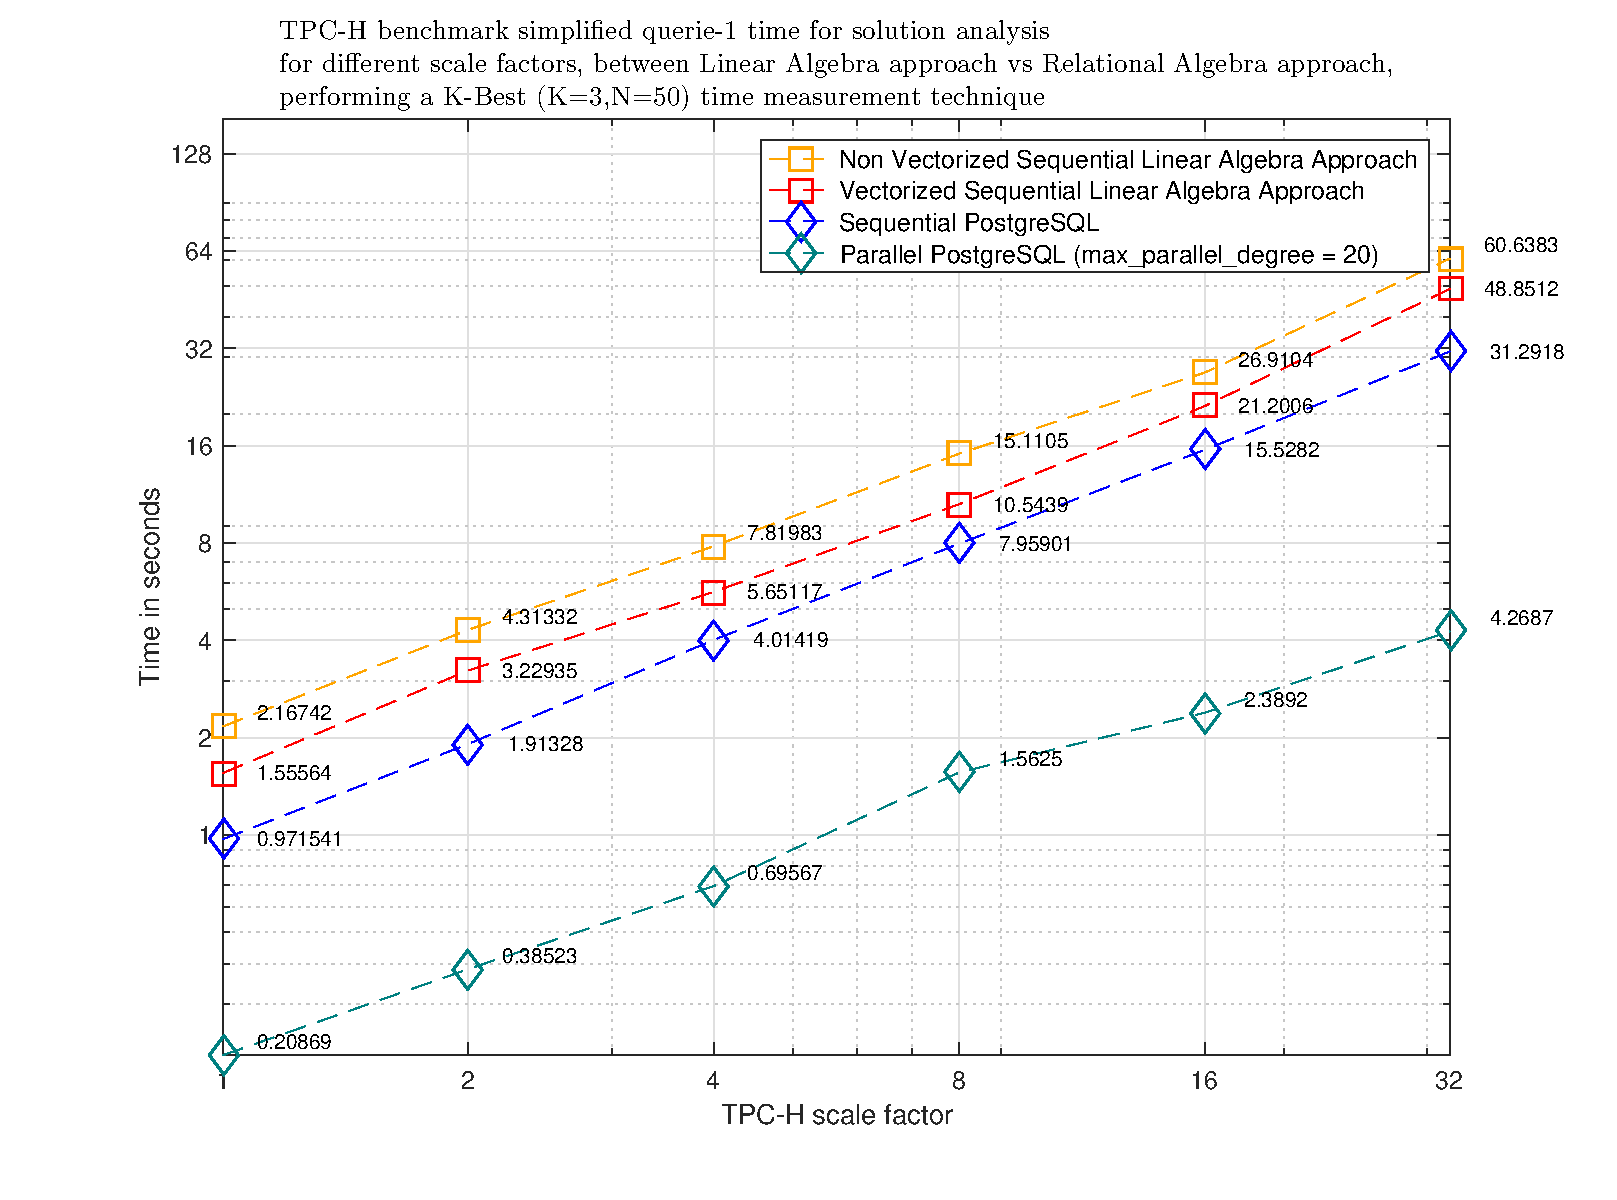
\includegraphics[width=1\columnwidth]{eps/TIME_LA_vs_RA_1st.eps}
\label{fig:time_la_vs_ra}
\end{figure}





\section{Hardware Characterization}
\indent
\par The platform used by us for our study at Search6 is a dual-socket system equipped with two Intel\textsuperscript{\textregistered} Ivy Bridge processors. The system, referenced as compute node 652-1, has two Intel\textsuperscript{\textregistered} Xeon\textsuperscript{\textregistered} E5-2670v2 (Ivy Bridge architecture) and features 64 GB of DDR3 RAM, supported at a frequency of XXXX MHz divided in 4 memory channels.

\begin{table}[H]
\centering
  \begin{tabular}{ | L{3.5cm} | R{5cm} | }
  
    \hline
    System & compute-652-1 \\ \hline \hline
        \# CPUs & 2\\ \hline
    CPU & Intel\textsuperscript{\textregistered} Xeon\textsuperscript{\textregistered} E5-2670v2\\ \hline 
    Architecture & Ivy Bridge \\ \hline 
    \# Cores per CPU & 10 \\ \hline 
    \# Threads per CPU & 20\\ \hline 
    Clock Freq. & 2.5 GHz\\ \hline \hline 
    L1 Cache & 320KB \newline 32KB per core\\ \hline 
    L2 Cache & 2560KB  \newline  256KB per core \newline\\ \hline 
    L3 Cache & 25600KB \newline shared \\ \hline \hline 
    Inst. Set Ext. & SSE4.2 \& AVX \\ \hline 
        \#Memory Channels & 4\\ \hline \hline

    Vendors Announced Peak Memory BW & 59.7 GB/s\\ \hline
    Measured\footnote{Stream Benchamrk} Peak Memory BW & 58.5GB/s\\ \hline
  \end{tabular}
     \caption{Architectural characteristics of the two evaluation platforms.}
     \label{table:characterization}
\end{table}


\section{Hardware Characterization}
\indent
\par The platform used by us for our study at Search6 is a dual-socket system equipped with two Intel\textsuperscript{\textregistered} Ivy Bridge processors. The system, referenced as compute node 652-1, has two Intel\textsuperscript{\textregistered} Xeon\textsuperscript{\textregistered} E5-2670v2 (Ivy Bridge architecture) and features 64 GB of DDR3 RAM, supported at a frequency of XXXX MHz divided in 4 memory channels.

\begin{table}[H]
\centering
  \begin{tabular}{ | L{3.5cm} | R{5cm} | }
  
    \hline
    System & compute-652-1 \\ \hline \hline
        \# CPUs & 2\\ \hline
    CPU & Intel\textsuperscript{\textregistered} Xeon\textsuperscript{\textregistered} E5-2670v2\\ \hline 
    Architecture & Ivy Bridge \\ \hline 
    \# Cores per CPU & 10 \\ \hline 
    \# Threads per CPU & 20\\ \hline 
    Clock Freq. & 2.5 GHz\\ \hline \hline 
    L1 Cache & 320KB \newline 32KB per core\\ \hline 
    L2 Cache & 2560KB  \newline  256KB per core \newline\\ \hline 
    L3 Cache & 25600KB \newline shared \\ \hline \hline 
    Inst. Set Ext. & SSE4.2 \& AVX \\ \hline 
        \#Memory Channels & 4\\ \hline \hline

    Vendors Announced Peak Memory BW & 59.7 GB/s\\ \hline
    Measured\footnote{Stream Benchamrk} Peak Memory BW & 58.5GB/s\\ \hline
  \end{tabular}
     \caption{Architectural characteristics of the two evaluation platforms.}
     \label{table:characterization}
\end{table}


\section{Hardware Characterization}
\indent
\par The platform used by us for our study at Search6 is a dual-socket system equipped with two Intel\textsuperscript{\textregistered} Ivy Bridge processors. The system, referenced as compute node 652-1, has two Intel\textsuperscript{\textregistered} Xeon\textsuperscript{\textregistered} E5-2670v2 (Ivy Bridge architecture) and features 64 GB of DDR3 RAM, supported at a frequency of XXXX MHz divided in 4 memory channels.

\begin{table}[H]
\centering
  \begin{tabular}{ | L{3.5cm} | R{5cm} | }
  
    \hline
    System & compute-652-1 \\ \hline \hline
        \# CPUs & 2\\ \hline
    CPU & Intel\textsuperscript{\textregistered} Xeon\textsuperscript{\textregistered} E5-2670v2\\ \hline 
    Architecture & Ivy Bridge \\ \hline 
    \# Cores per CPU & 10 \\ \hline 
    \# Threads per CPU & 20\\ \hline 
    Clock Freq. & 2.5 GHz\\ \hline \hline 
    L1 Cache & 320KB \newline 32KB per core\\ \hline 
    L2 Cache & 2560KB  \newline  256KB per core \newline\\ \hline 
    L3 Cache & 25600KB \newline shared \\ \hline \hline 
    Inst. Set Ext. & SSE4.2 \& AVX \\ \hline 
        \#Memory Channels & 4\\ \hline \hline

    Vendors Announced Peak Memory BW & 59.7 GB/s\\ \hline
    Measured\footnote{Stream Benchamrk} Peak Memory BW & 58.5GB/s\\ \hline
  \end{tabular}
     \caption{Architectural characteristics of the two evaluation platforms.}
     \label{table:characterization}
\end{table}


\section{Hardware Characterization}
\indent
\par The platform used by us for our study at Search6 is a dual-socket system equipped with two Intel\textsuperscript{\textregistered} Ivy Bridge processors. The system, referenced as compute node 652-1, has two Intel\textsuperscript{\textregistered} Xeon\textsuperscript{\textregistered} E5-2670v2 (Ivy Bridge architecture) and features 64 GB of DDR3 RAM, supported at a frequency of XXXX MHz divided in 4 memory channels.

\begin{table}[H]
\centering
  \begin{tabular}{ | L{3.5cm} | R{5cm} | }
  
    \hline
    System & compute-652-1 \\ \hline \hline
        \# CPUs & 2\\ \hline
    CPU & Intel\textsuperscript{\textregistered} Xeon\textsuperscript{\textregistered} E5-2670v2\\ \hline 
    Architecture & Ivy Bridge \\ \hline 
    \# Cores per CPU & 10 \\ \hline 
    \# Threads per CPU & 20\\ \hline 
    Clock Freq. & 2.5 GHz\\ \hline \hline 
    L1 Cache & 320KB \newline 32KB per core\\ \hline 
    L2 Cache & 2560KB  \newline  256KB per core \newline\\ \hline 
    L3 Cache & 25600KB \newline shared \\ \hline \hline 
    Inst. Set Ext. & SSE4.2 \& AVX \\ \hline 
        \#Memory Channels & 4\\ \hline \hline

    Vendors Announced Peak Memory BW & 59.7 GB/s\\ \hline
    Measured\footnote{Stream Benchamrk} Peak Memory BW & 58.5GB/s\\ \hline
  \end{tabular}
     \caption{Architectural characteristics of the two evaluation platforms.}
     \label{table:characterization}
\end{table}



 
%---------------------------------------------------------------------------------------
%	REFERENCE LIST
%--------------------------------------------------------------------------------------


\bibliographystyle{plain}
\bibliography{biblio}

%---------------------------------------------------------------------------------------
\end{multicols}
\end{document}



